Operační systém je zpravidla tvořen tzv. \textbf{jádrem} (kernel), \textbf{ovladači I/O zařízení} (driver), příkazovým procesorem (shell) a podpůrnými systémovými programy.
\begin{itemize}
	\item \textbf{Jádro} -- po \textbf{zavedení} do paměti \textbf{řídí} činnost počítače, poskytuje procesům služby a řeší správu prostředků a správu procesů.
	\item \textbf{Ovladač} -- zvláštní (pod)program pro \textbf{ovládání konkrétního zařízení} standardním způsobem. Použití strategie s ovladači umožňuje snadnou konfigurovatelnost technického vybavení.
	\item \textbf{Příkazový procesor} -- program, který \textbf{umožňuje} uživatelům \textbf{zadávat příkazy} ve speciálním, obvykle jednoduchém jazyce.
	\item \textbf{Podpůrné programy} -- do této kategorie jsou mnohdy zahrnovány i překladače (jazyk C v OS UNIX) a sestavující programy. Stojí na stejném místě jako aplikační programy.
\end{itemize}

\subsection{Jádro}
Jádro se zpravidla dělí na dvě podstatné části:
\begin{enumerate}
	\item \textbf{Správa procesů} -- řeší problematiku aktivování a deaktivování procesů podle jejich priority resp. požadavků na prostředky (prakticky není u jednoduchých OS)
	\item \textbf{Správa prostředků} -- zajištuje činnost I/O zařízení, přiděluje paměť, případně procesory. Velmi důležitou částí správy prostředků je \textbf{správa souborů} -- způsob ukládání souborů a přístupu k nim. Moderní OS zajištují jednotný pohled na soubory a zařízení. Zařízení jsou považovány za soubory se speciálním jménem.
\end{enumerate}

\subsection{Generické komponenty OS} % https://publi.cz/books/11/04.html

\begin{itemize}
	\item Správa procesorů
	\item Správa procesů (proces – činnost řízená programem)
	\item Správa vnitřní (hlavní) paměti
	\item Správa souborů 
	\item Správa I/O systému
	\item Správa vnější (sekundární) paměti 
	\item Networking, distribuované systémy
	\item Systém ochran
	\item Interpret příkazů
\end{itemize}
\begin{figure}[H]
\centering
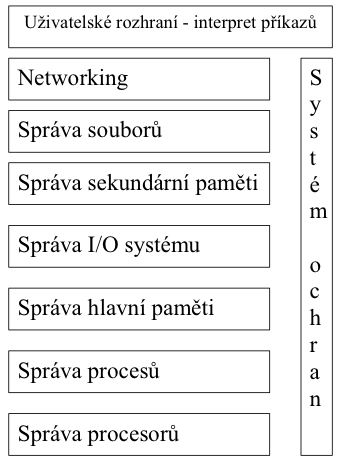
\includegraphics[width=0.4\textwidth]{assets/3_gen_komp_os}
\end{figure}

\subsubsection{Správa procesorů/procesů}
Správce procesoru má tyto funkce:
\begin{itemize}
	\item sleduje prostředek (procesor a stav procesů),
	\item rozhoduje, komu bude dána možnost užít procesor,
	\item přiděluje procesoru prostředek, tj. procesor,
	\item požaduje vrácení prostředku (procesoru).
\end{itemize}

Pojem \textbf{proces} (task) je nějaká činnost řízená programem. Proces potřebuje pro svou realizaci jisté zdroje:
\begin{itemize}
	\item dobu procesoru,
	\item paměť,
	\item I/O zařízení, atd.
\end{itemize}
OS je z hlediska \textbf{správy procesů} zodpovědný za:
\begin{itemize}
	\item vytváření a rušení procesů,
	\item potlačení a obnovení procesů,
	\item poskytnutí mechanismů pro synchronizaci procesů a pro komunikaci mezi procesy.
\end{itemize}
OS je z hlediska \textbf{správy procesorů} zodpovědný za výběr procesu běžícího na volném procesoru.

\subsubsection{Správa (hlavní, operační) paměti}
Jedná se o úložiště připravených tj. rychle dostupných dat sdílených procesorem a I/O zařízeními. Hlavní paměť je pole samostatně adresovatelných slov nebo bytů, zpravidla energeticky závislá.\\
OS je z hlediska správy \textbf{(hlavní) paměti} odpovědný za:
\begin{itemize}
	\item vedení přehledů kdo a kterou část paměti v daném okamžiku využívá,
	\item rozhodování, kterému procesu uspokojit jeho požadavek na prostor paměti po uvolnění,
	\item přidělování a uvolňování paměti dle potřeby,
	\item řízení virtuální paměti.
\end{itemize}
Z hlediska těchto zodpovědností správce operační paměti:
\begin{itemize}
	\item udržuje přehled o přidělované a volné paměti,
	\item ve spolupráci se správou procesů rozhoduje o tom, kterému procesu, kolik, kde a kdy má přidělit operační paměť,
	\item provádí přidělení volné části paměti,
	\item určuje strategii odnímání dříve přidělené operační paměti procesům (opět po předchozí domluvě se správou procesů).
\end{itemize}

\subsubsection{Správa I/O systému}
Správce periferních (I/O systému) má tyto funkce:
\begin{itemize}
	\item sleduje stav prostředků (periferních zařízení, jejich řídících jednotek),
	\item rozhoduje o efektivním způsobu přidělování prostředku -- periferního zařízení,
	\item přiřazuje prostředek (periferní zařízení) a zahajuje I/O operaci,
	\item požaduje navrácení prostředku.
\end{itemize}
Z hlediska funkce OS lze správce I/O systému chápat jako:
\begin{itemize}
	\item úložiště vyrovnávacích pamětí,
	\item univerzální rozhraní ovladače I/O zařízení,
	\item ovladače jednotlivých hardwarových I/O zařízení.
\end{itemize}
Do správy I/O systému patří i \textbf{správa vnější (sekundární) paměti}. Počítačový systém musí poskytnout pro zálohování hlavní paměti sekundární paměť (HDD, SSD). OS je z hlediska správny vnější (sekundární) paměti odpovědný za:
\begin{itemize}
	\item správu volné paměti,
	\item přidělování paměti,
	\item plánování činnosti disku.
\end{itemize}

\subsubsection{Správa souborů}
Správce souborů má tyto funkce:
\begin{itemize}
	\item sleduje prostředek (soubor), jeho umístění, užití, stav atd.,
	\item rozhoduje, komu budou prostředky \textbf{přiděleny}, realizuje požadavky na \textbf{ochranu informací uložených} v souborech a realizuje operace přístupu k souborům,
	\item \textbf{přiděluje} prostředek, tj. otevírá soubor,
	\item \textbf{uvolňuje} prostředek, tj. uzavírá soubor.
\end{itemize}
Pod pojmem soubor chápeme jak programy, tak data. OS je z hlediska správy souborů odpovědný za:
\begin{itemize}
	\item vytváření a rušení souborů,
	\item vytváření a rušení adresářů (katalogů, složek),
	\item podporu primitivních \textbf{operací} pro manipulaci se soubory a adresáři,
	\item archivování souborů na energeticky nezávislí média.
\end{itemize}
\subsubsection{Networking, distribuované systémy}
Distribuovaný systém je \textbf{kolekce procesorů}, které \textbf{nesdílejí} ani \textbf{fyzickou paměť} ani \textbf{hodiny}, synchronizující činnost procesoru. Každý procesor má svoji \textbf{lokální paměť} a \textbf{lokální hodiny}. Procesory distribuovaného systému jsou \textbf{propojeny} komunikační sítí. Komunikace jsou řízeny protokoly. Distribuovaný systém uživateli zprostředkovává přístup k různým zdrojům systému.

\subsubsection{Systém ochran}
Jsou to mechanismy pro \textbf{řízení přístupu} k \textbf{systémovým} a \textbf{uživatelským zdrojům}. Systém ochran musí:
\begin{itemize}
	\item \textbf{rozlišovat} mezi \textbf{autorizovaným} a \textbf{neautorizovaným} použitím,
	\item specifikovat problém vnucovaného řízení,
	\item poskytnout prostředky pro své prosazení.
\end{itemize}

\subsubsection{Uživatelské rozhraní - interpret příkazů}
Interpret příkazů je program, umožnující vykonávat příkazy pro:
\begin{itemize}
	\item správu a vytváření procesů -- služby OS poskytované interperetem příkazů slouží k \textbf{provedení programu}, tj. k schopnosti OS zavést program do hlavní paměti a spustit jeho běh,
	\item ovládání I/O zařízení -- uživatelský program \textbf{nesmí} provádět I/O operace \textbf{přímo}, OS musí poskytovat prostředky k provádění I/O operací,
	\item správu sekundární paměti -- manipulace se systémem souborů, schopnost číst, zapisovat, vytvářet a rušit soubory,
	\item správu hlavní paměti,
	\item zpřístupňování souborů,
	\item ochranu -- tj. d\textbf{etekci chyb v procesoru} a \textbf{paměti}, I/O zařízeních a v programech uživatelů pro zajištění správnosti výpočtu,
	\item práci v síti -- \textbf{výměna informací} mezi procesy realizována buďto v rámci jednoho počítače nebo mezi různými počítači pomocí sítě, tj. implementace sdílenou pamětí nebo předávání zpráv.
\end{itemize}
Uživatelská rozhraní jsou realizovaná \textbf{znakově} (někdy označované řádkově) nebo \textbf{graficky}. Znakově orientovaným interpretům zadáváme příkazy pomocí klíčových slov, graficky orientovaným pomocí poklepání myši nebo dotykem na dotykové obrazovce na ikonu, pomocí dialogů apod.

\subsubsection{Vnitřní služby operačního systému}
Vnitřní služby OS \textbf{nejsou} určeny k tomu, aby \textbf{pomáhaly uživateli}, v prvé řadě slouží pro \textbf{zabezpečení efektivního provozu systému}, tj. slouží pro:
\begin{itemize}
	\item Přidělování prostředků (zdrojů) mezi více souběžně operujících uživatelů nebo úloh.
	\item Účtování a udržování přehledu o tom, kolik jakých zdrojů systému který uživatel používá. Cílem je účtování za služby a sběr statistik pro plánování.
	\item Ochranu tj. péči o to, aby veškerý přístup k systémovým zdrojům byl pod kontrolou.
\end{itemize}
Vnitřní služby OS jsou obecně \textbf{realizovány souborem systémových programů} vytvářejících určité systémové struktury tzv. virtuální stroje. Typickými službami jsou programy pro:
\begin{itemize}
	\item práci se soubory, editaci souborů, katalogizaci souborů, modifikaci souborů,
	\item získávání, definování a údržbu systémových informací,
	\item podporu jazykových prostředí,
	\item zavádění a provádění programů,
	\item komunikace a řízení aplikačních programů.
\end{itemize}

\subsection{Struktura OS podle jádra}
\begin{itemize}
	\item Monolitická jádra (monolithic kernel)
	\item Otevřené systémy (Open oystems)
	\item Microkernel
\end{itemize}
\subsubsection{Monolitický OS}
OS je na jedno místě (v obrázku pod \uv{červenou čarou}). Aplikace používá dobře definované rozhraní systémového volání pro komunikaci s jádrem.
\begin{figure}[H]
\centering
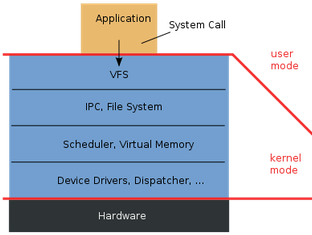
\includegraphics[width=0.7\textwidth]{assets/3_mon_os}
\end{figure}
Příklady OS -- Unix, Windows NT / XP, Linux, BSD.

Monolitické jádro je specifické pro komerční systémy.
\subsubsection*{Výhody}
\begin{itemize}
	\item[$+$] dobrý výkon
	\item[$+$] dobře pochopená koncepce
	\item[$+$] jednoduché pro vývojáře jádra
	\item[$+$] vysoká úroveň ochrany mezi aplikacemi
\end{itemize}
\subsubsection*{Nevýhody}
\begin{itemize}
	\item[$-$] žádná ochrana mezi komponentami jádra
	\item[$-$] není jednoduše a bezpečně rozšiřitelné jádro
	\item[$-$] celková struktura je ve výsledku komplikovaná, neexistující hranice mezi moduly jádra
\end{itemize}

\subsubsection{Otevřené Systémy}
Aplikace, knihovny i jádro jsou všechny v jednom adresovaném prostoru.

Příklady OS -- MS--DOS, Mac OS 9 a starší, Windows ME, 98, 95, 3.1, Palm OS.

Tato koncepce bývala velmi běžná.
\begin{figure}[H]
\centering
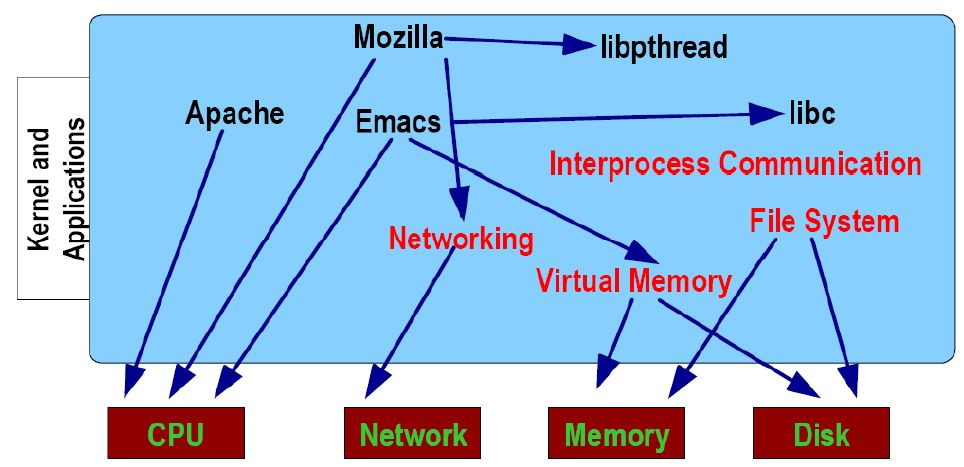
\includegraphics[width=0.7\textwidth]{assets/3_open_sys}
\end{figure}
\subsubsection*{Výhody}
\begin{itemize}
	\item[$+$] velmi dobrý výkon
	\item[$+$] velmi dobře rozšiřitelné
	\item[$+$] výhodné pro jednouživatelské OS
\end{itemize}
\subsubsection*{Nevýhody}
\begin{itemize}
	\item[$-$] žádná ochrana mezi jádrem a aplikacemi
	\item[$-$] nepříliš stabilní
	\item[$-$] skládání rozšíření může vést k nepředvídatelnému chování
\end{itemize}

\subsubsection{Microkernel OS}
Filosofie návrhu -- chráněné jádro obsahuje pouze minimálné (malou, čistou, logickou) množinu abstrakcí:
\begin{itemize}
	\item procesy a vlákna
	\item virtuální paměť
	\item komunikace mezi procesy
\end{itemize}
Všechno ostatní jsou server--procesy běžící na uživatelské úrovni.

Příklady OS -- Marc, Chorus, QNX, GNU Hurd

Zkušenosti s tímto návrhem jsou smíšené.
\begin{figure}[H]
\centering
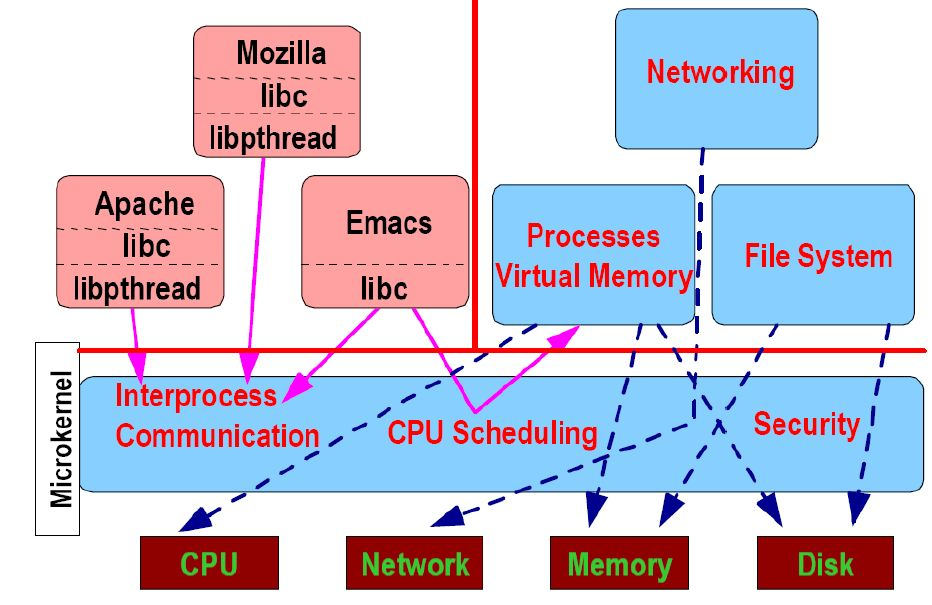
\includegraphics[width=0.7\textwidth]{assets/3_microkernel}
\end{figure}
\subsubsection*{Výhody}
\begin{itemize}
	\item[$+$] přidáním server--procesu se rozšíří funkcionalita OS
	\item[$+$] jádro nespecifikuje prostředí OS
	\item[$+$] servery na uživatelské úrovni se nemusí zabývat hardwarem
	\item[$+$] silná ochrana OS i sám proti sobě (části OS jsou oddělené servery)
	\item[$+$] jednoduché rozšíření na distribuovaný nebo multiprocesorový systém
\end{itemize}
\subsubsection*{Nevýhody}
\begin{itemize}
	\item[$-$] výkon (systémová volání, viz příklad pod touto kapitolou)
	\item[$-$] špatná minulost
\end{itemize}

\subsubsection{Příklad systémového volání}
\begin{figure}[H]
\centering
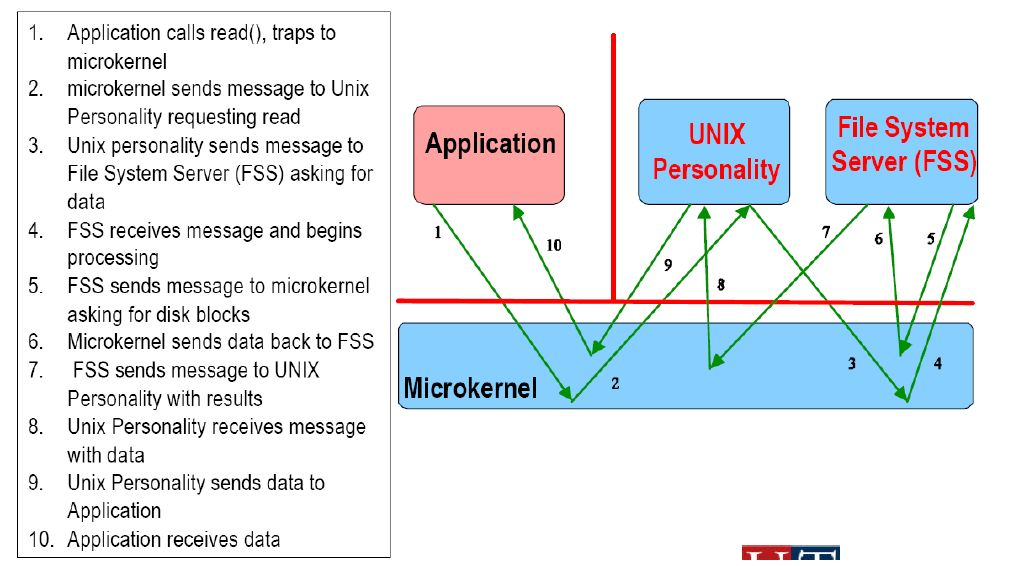
\includegraphics[width=1\textwidth]{assets/3_sys_call}
\end{figure}